\documentclass[a4paper, 11pt, oneside]{extbook}\usepackage[T1]{fontenc}
\usepackage[utf8x]{inputenc}
\usepackage[italian]{babel} %Lingua italiana per gli standard e gli accenti
\usepackage{geometry}
\usepackage{courier}
\usepackage{pdfpages}
\usepackage{amssymb}
%\usepackage{amsthm}
\usepackage{amsmath}
\usepackage{tikz}
\usepackage[bookmarks]{hyperref}
\newgeometry{
	left=   1.5 in,
	bottom= 1.5 in,
	right=  1 in,
	top=    1 in
}

\usepackage{fancyhdr}

% Grafica
\usepackage{graphicx,pstricks}
\usepackage{graphics}
\usepackage{subfigure}

%
%Algorithm
\usepackage{algorithm}
\usepackage[noend]{algpseudocode}

\setlength\headheight{44.2pt}
%Page Style
\usepackage{setspace}
%\setstretch{2.5} 
\doublespace
%
%%\cfoot{\thepage}
%\lhead[]{}
%\rhead[]{\leftmark}

\pagestyle{fancy}{
%	\lhead{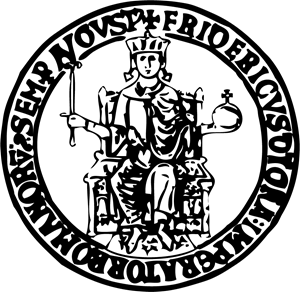
\includegraphics[scale=0.3]{img/logo.png}}
	%	\rhead{\footnotesize{\leftmark}}
	\rhead{\footnotesize{\leftmark}}
	%	\rfoot{\thepage}
}

%\fancyfoot[CE,CO]{\leftmark}
%\fancyfoot[LE,RO]{\thepage}
\renewcommand{\footrulewidth}{1pt}
\linespread{1}

%Other
\usepackage{comment}
\usepackage{amsmath}

%Testo riempitivo
\usepackage{lipsum}




\begin{document}
	\begin{titlepage}
	\begin{center}
		\vspace*{1cm}
		
		\Huge
		\textbf{Università degli Studi di Napoli \\ "Federico II"}
		
		\vspace{0.5cm}
		\LARGE
		Scuola Politecnica e delle Scienze di Base\\
		Corso di Laurea Magistrale in Ingegneria Informatica
		
		\vspace{1.5cm}
		
		\textbf{Giuseppe Francesco Di Cecio - M63001211}
		\\
		\textbf{Nicola D'Ambra - M63001223}
		\\
		\textbf{Emma Melluso - M63001176}
		
		\vspace{2cm}
		
		
		
		\vspace{0.5cm}
		\LARGE
		\textbf{Elaborato di \textit{Impianti di Elaborazione}}
		\vfill
		
		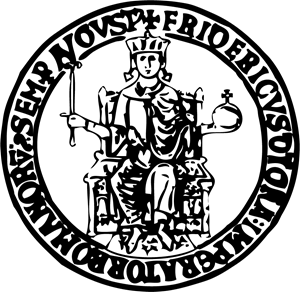
\includegraphics[width=0.2\textwidth]{img/logo.png}
		
		\Large
		Università degli Studi di Napoli \textit{Federico II}\\
		Napoli\\
		A.A 2020/2021
		
	\end{center}
\end{titlepage}

	\frontmatter						%Numerazione romana
	

	{\setstretch{1.5}					%Indice
		\tableofcontents
	}
	
	\backmatter							%Inizio numerazione capitoli
	\mainmatter							%Numerazione pagine
	\chapter{Workload Characterization}
Il dataset di partenza è composto da \textbf{3000 righe} e \textbf{24 colonne}, ciascuna delle quali rappresenta uno dei parametri del sistema oggetto di studio. Si tratta di parametri caratterizzanti l'esecuzione di vari Threads su un sistema operativo.
\\In particolar modo le colonne con prefisso $Vm$ rappresentano informazioni sulla memoria virtuale occupata e utilizzata dai Threads, mentre le altre colonne rappresentano informazioni di carattere generale, come memoria libera, numero di threads, pagine inattive ecc.

\section{Filtraggio}

\subsection{Colonne Identiche}
Innanzitutto osservando il workload e effettuando un grafico delle distribuzioni è possibile rendersi conto della presenza di ben 4 colonne costanti:
\begin{itemize}
	\item \textbf{Active}
	\item \textbf{AnonPages}
	\item \textbf{AvbLatency}
	\item \textbf{Error}
\end{itemize}
Tali colonne in quanto costanti non spiegano varianza, dunque possono essere tranquillamente trascurate ai fini dell'analisi.
\\Osservando le distribuzioni dei parametri \textbf{WriteBack} e \textbf{MemFree} si sono notate alcune caratteristiche comuni. Per avere una maggiore chiarezza si è preferito calcolare la matrice delle correlazioni su questi due parametri.
\begin{figure}[H]
	\centering
	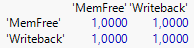
\includegraphics{img/hw1/correlazione_mem_writeback.png}
	\caption{\textit{Matrice di correlazione tra MemFree e WriteBack}}
\end{figure}
Osservando la matrice appare evidente che le due colonne sono esattamente identiche, fornendo quindi la stessa informazione. Per questo motivo si è deciso di trascurare una delle due, in particolare quella di WriteBack.
\\Le 24 colonne iniziali sono state ridotte a 19 colonne, riducendo il dataset di un numero di osservazioni pari a:
\begin{equation}
	n_{dati} = 3.000 \times (24 - 19) = 15.000
\end{equation}

\subsection{Outlier}
Gli outliers sono valori anomali all'interno dell'insieme di osservazioni, in altre parole sono valori che si discostano notevolmente dagli altri valori dell'insieme. 
Essendo valori anomali la loro frequenza di occorrenza è bassa rispetto agli altri valori e ciò li porta ad essere identificati all'esterno del range interquartile. 
In alcuni casi gli outlier possono essere eliminati ma ciò è possibile solo a monte di una analisi accurata. Tali valori infatti influiscono sulle analisi statistiche in modo considerevole e non sempre rappresentano situazioni trascurabili per l'analisi da svolgere .
Osservando attraverso box plot e grafici di distribuzione l'andamento dei seguenti parametri :
\begin{itemize}
	\item \textbf{VmSize} (quanta memoria virtuale utilizza l'intero processo);
	\item \textbf{VmHWM} (di quanta RAM il processo necessita al massimo);
	\item \textbf{VmRSS} (quanta RAM il processo sta correntemente usando);
	\item \textbf{VmPTE} (quanta memoria Kernel è occupata dalle entries della tabella delle pagine);
\end{itemize}
\begin{figure}[H]
	\centering
	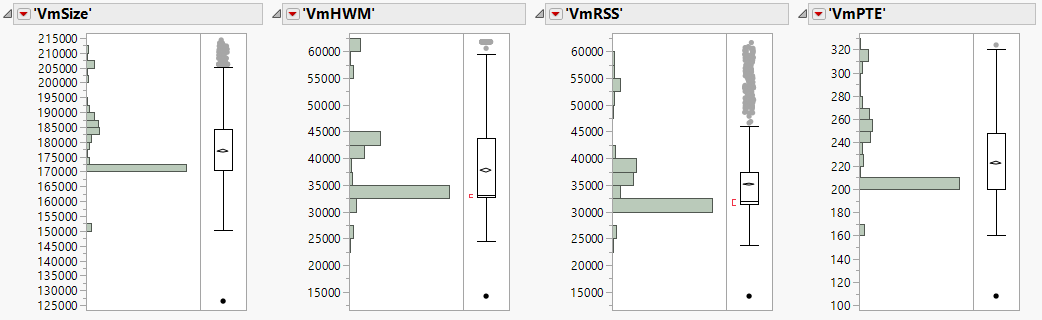
\includegraphics[width=1\textwidth]{img/hw1/outlier_vm.png}
	\caption{\textit{Grafici di distribuzione di VmSize, VmHWM, VmRSS, VmPTE}}
\end{figure}
Si è notato che essi presentano un outlier isolato (in basso ad ogni grafico) in comune associato alla prima riga del dataset. Analizzando gli altri parametri (\textit{MemFree}, \textit{Dirty}, \textit{PageTables}, \textit{Buffer}, ...) è stato possibile evidenziare che anche per la maggior parte di essi lo è, ma non è un punto isolato. 
\\L'ipotesi fatta è che con molta probabilità le prime righe del dataset (da 0 a 100 circa), rappresentano la fase di avvio del processo e l'outlier oggetto di studio è la prima istanza di questa fase. Dato che l'obiettivo della caratterizzazione del workload è quello di analizzare le prestazioni a regime del sistema oggetto di studio (in questo caso), si è deciso di trascurare quel singolo outlier. Tuttavia è bene notare che in ogni caso le informazioni riguardo questa fase di avvio non saranno del tutto perse dato che è stato rimosso un singolo punto e non tutti i punti che la rappresentano.
\\
\vspace{0.5cm}
\\
Un secondo outlier che può essere agevolmente rimosso è la riga 512 in cui il parametro \textbf{Slab} assume valore 4. 
\begin{figure}[H]
	\centering
	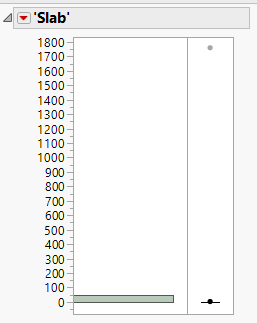
\includegraphics[width=0.4\textwidth]{img/hw1/outlier_slab1.png}
	\caption{\textit{Grafico di distribuzione di Slab}}
\end{figure}
Oltre ad avvicinarsi molto al valore medio assunto da Slab (zero), esso risulta essere un outlier solo per il parametro stesso dato che per gli altri è un valore compreso tra i quartili. Una sua rimozione quindi non influenza gli indici di caratterizzazione sintetica dei parametri del workload complessivo.
\\
\vspace{0.5cm}
\\
Un terzo outlier è il valore 1760 del parametro \textit{Slab}, associato alla riga 90 del workload.
\begin{figure}[H]
	\centering
	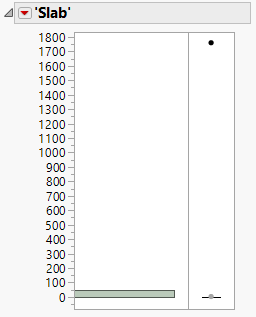
\includegraphics[width=0.4\textwidth]{img/hw1/outlier_slab2.png}
	\caption{\textit{Grafico di distribuzione di Slab}}
\end{figure}
Rispetto al precedente, tale outlier richiede un' analisi più approfondita visto che influenza significativamente l'andamento di parametri quali \textit{Mapped} e \textit{PageTables}. Per descrivere meglio la dipendenza tra questi parametri si può effettuare un grafico tra il numero dell'osservazione e il valore assunto da \textit{Mapped}, analogo discorso con \textit{PageTables}.	
\begin{figure}[H]
	\centering   
	\subfigure{	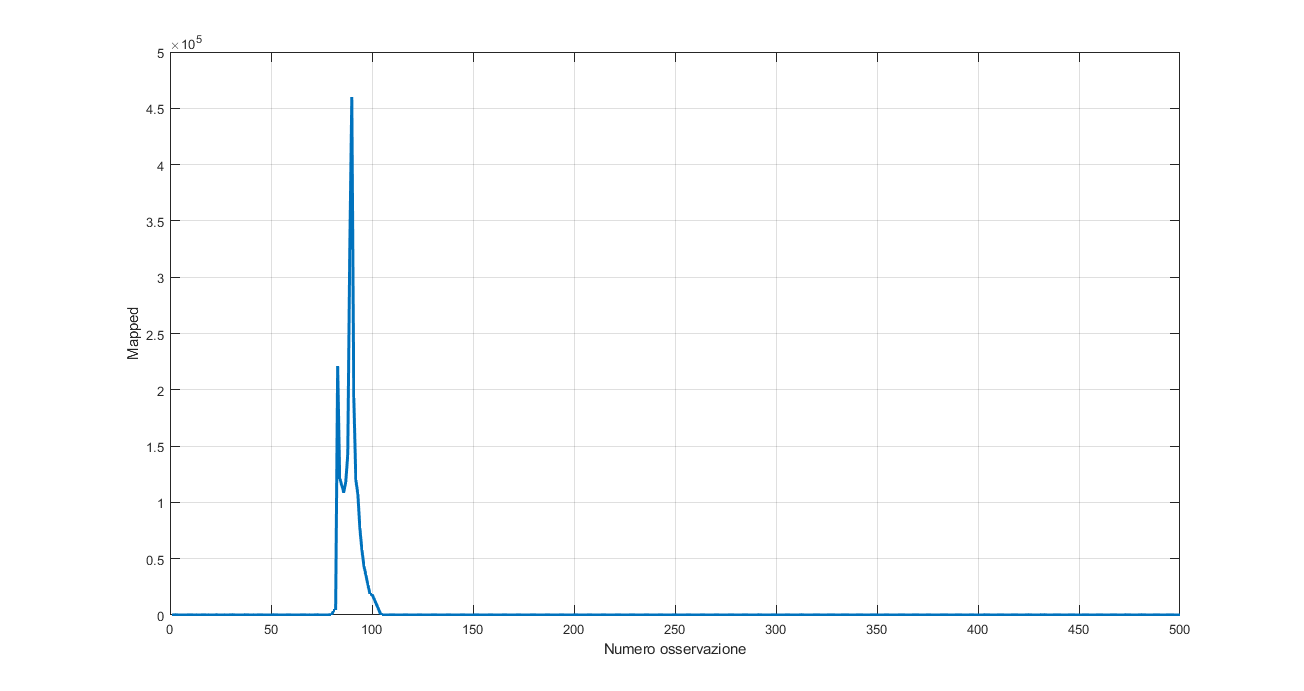
\includegraphics[width=\textwidth]{img/hw1/mapped.png}}
	\caption{\textit{Grafico tra numero di osservazione e valore assunto dal parametro Mapped}}
	\subfigure{	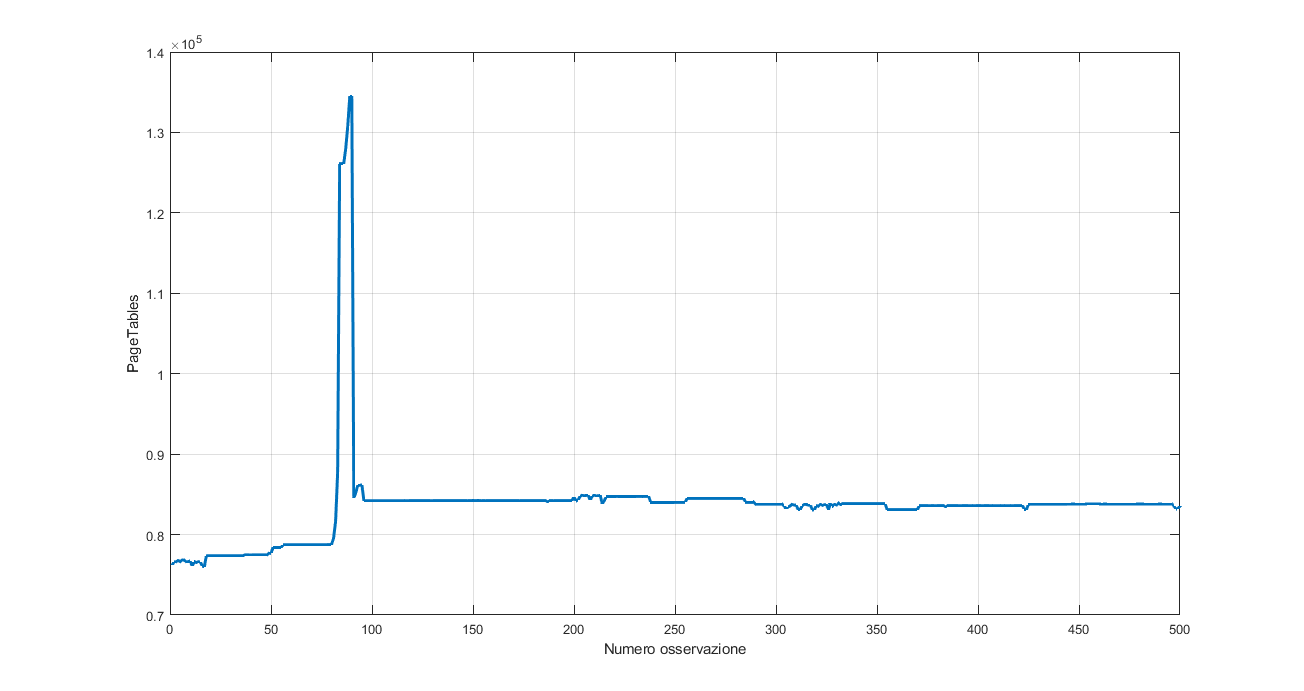
\includegraphics[width=\textwidth]{img/hw1/pagetables.png}}	
	\caption{\textit{Grafico tra numero di osservazione e valore assunto dal parametro PageTables}}
\end{figure}
Si nota che in corrispondenza (in realtà nell'osservazione appena precedente) dell'outlier del parametro \textit{Slab} i due parametri sopra indicati hanno un picco, durante la fase di avvio del sistema.
\\Lo Slab si riferisce ad un particolare meccanismo di allocazione/deallocazione della memoria nel Kernel. Dato che influenza in particolar modo altri parametri si è preferito non trascurarlo.\\
In conclusione sono stati eliminati dal dataset solo 2 outlier che corrispondono a 38 osservazioni. Quindi il dataset è stato ridotto in totale di 15.038 elementi, provocando una diminuzione dei dati iniziali di poco più del $20\%$.
\newpage

\section{PCA}
A seguito del filtraggio il dataset risulta ridotto grazie alla rimozione di alcune colonne che non esprimevano varianza e alcune righe rappresentanti outlier trascurabili.
\\Su questo dataset si possono quindi iniziare a fare le prime considerazioni.
\\Utilizzando la tecnica della \textit{Principal Component Analysis} il dataset può essere estremamente ridotto, sfruttando solo le \textit{Componenti Principali} che mantengono più varianza. Il risultato della PCA è quindi:
\begin{figure}[H]
	\centering
	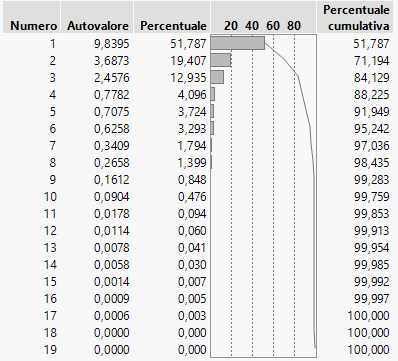
\includegraphics{img/hw1/pca.png}
	\caption{\textit{PCA applicata al dataset filtrato}}
\end{figure}
La scelta del numero di componenti principali ricade in particolar modo sulla devianza che quelle componenti mantengono rispetto al dataset reale. Inoltre essa dipende anche dal tipo di osservazioni ed esperimento che è stato effettuato.
\\In questo caso la scelta è ricaduta sul prendere 5 componenti principali poiché rappresentano il 92\% della devianza totale. Esso rappresenta un valore abbastanza elevato, ma è stato scelto per mantenersi in una regione di tolleranza durante la clusterizzazione. 
\\Anche se il workload sintentico verrà costruito considerando 5 componenti principali, in seguito sono riportati i risultati di PCA e clusterizzazione anche nel caso in cui fosse stato scelto un numero diverso di componenti principali, ovvero:
\begin{itemize}
	\item Prendere 4 PC
	\begin{equation*}
		DEV_{PCA-MANTENUTA} \approx 88 \%
	\end{equation*}
	\item Prendere 5 PC
	\begin{equation*}
			DEV_{PCA-MANTENUTA} \approx 92 \%
	\end{equation*}
	\item Prendere 6 PC
	\begin{equation*}
			DEV_{PCA-MANTENUTA} \approx 95 \%
	\end{equation*}
\end{itemize}
Per ognuno di questi 3 insiemi di Principal Components è stata effettuata la procedura di clustering .

\section{Clustering}
Il clustering è una tecnica che consiste nel raggruppare osservazioni "simili" tra loro. La similitudine tra un elemento e un cluster, o tra un cluster e un altro cluster, può essere calcolata secondo varie tecniche. In questa analisi si è preferito utilizzare il \textbf{metodo di Ward}, il quale pesa la distanza tra due cluster in relazione al numero di elementi che li compongono.
\\Dati due cluster P e Q (un elemento non appartenente ad un cluster, può essere visto come un cluster di dimensione 1), sia $|P|$ la cardinalità di $P$, analogo con $|Q|$, e sia $\bar{x}_p$ il centroide di $P$, analogo con $\bar{x}_q$, la distanza tra $P$ e $Q$ viene calcolata come:
\begin{equation*}
	d(P,Q) = 2 \dfrac{|P| \; |Q|}{|P| + |Q|} ||\bar{x}_p - \bar{x}_q ||^2
\end{equation*}
Per ogni raggruppamento viene poi scelto una singola osservazione che la rappresenta, riducendo quindi il numero di righe del dataset pari al numero di cluster scelti durante l'analisi.
\\Il numero di cluster da scegliere può dipendere da vari fattori:
\begin{itemize}
	\item Omogeneità dei cluster: i cluster devono raggruppare un numero di osservazioni quanto il più possibile omogeneo rispetto agli altri cluster. Avere un cluster con un numero di elementi di vari ordini di grandezza rispetto ad un altro cluster non sempre può portare a buoni risultati (in termini di devianza).
	\item Devianza mantenuta: a seguito della PCA parte della devianza nei dati viene persa. Dato che il clustering viene effettuato sulle \textit{Componenti Principali} allora esso produce un'ulteriore perdita di devianza nel risultato finale.
\end{itemize}
\subsubsection{Devianza Persa}
Per effettuare il calcolo della devianza totale persa persa bisogna prima calcolare la devianza intra-cluster (la somma delle devianze per ogni cluster) e sulla base di questa si può calcolare la quantità richiesta.
\\Matematicamente, definita $DEV_{PCA-PERSA}$ la devianza persa (in termini percentuali) a causa della PCA, viceversa $DEV_{PCA-MANTENUTA}$ la devianza mantenuta dalla PCA, e $DEV_{INTRA}$ la devianza intra-cluster, la devianza totale persa percentuale vale:
\begin{equation*}
	DEV_{PCA-LOST} + DEV_{INTRA}\times DEV_{PCA-MANTENUTA}
\end{equation*}
Essa può essere calcolata in MATLAB passando ad uno script i cluster, le componenti principali e il dataset iniziale.
\\ Per dare valore ai fattori sopra citati il clustering viene effettuato scegliendo un numero di cluster che varia da 6 a 16 (per ogni gruppo di componenti principali) su cui poi viene calcolata la devianza persa.
\newpage
 \subsection{4 Componenti Principali}
 Utilizzando le prime quattro PC si ha:
 \begin{figure}[H]
 	\centering   
 	\subfigure{	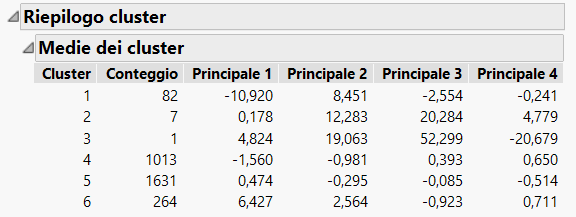
\includegraphics[width=0.30\textwidth]{Homework/Workload_Characterization/PCA_&_Clustering/4_Comp/Clustering/6_Cluster/Screen_Dati/Riepilogo.png}}
 	\subfigure{	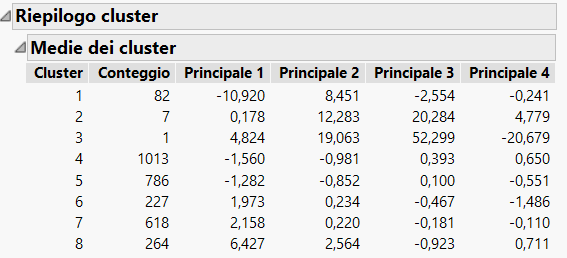
\includegraphics[width=0.30\textwidth]{Homework/Workload_Characterization/PCA_&_Clustering/4_Comp/Clustering/8_Cluster/Screen_Dati/Riepilogo.png}}
 	\subfigure{	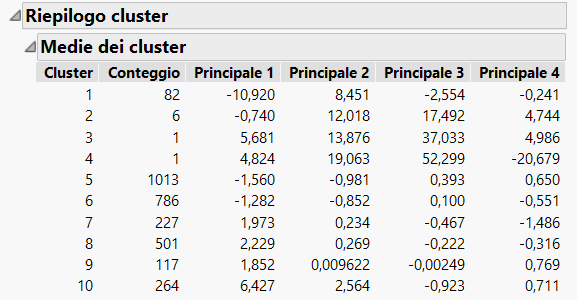
\includegraphics[width=0.30\textwidth]{Homework/Workload_Characterization/PCA_&_Clustering/4_Comp/Clustering/10_Cluster/Screen_Dati/Riepilogo.png}}
 	\subfigure{	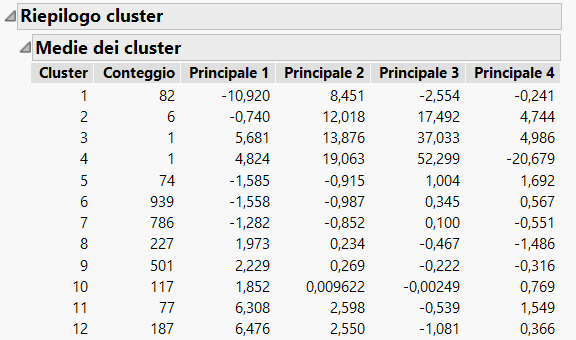
\includegraphics[width=0.30\textwidth]{Homework/Workload_Characterization/PCA_&_Clustering/4_Comp/Clustering/12_Cluster/Screen_Dati/Riepilogo.png}}
 	\subfigure{	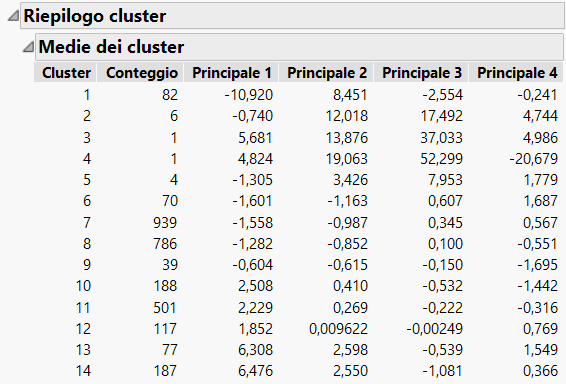
\includegraphics[width=0.30\textwidth]{Homework/Workload_Characterization/PCA_&_Clustering/4_Comp/Clustering/14_Cluster/Screen_Dati/Riepilogo.png}}
 	\subfigure{	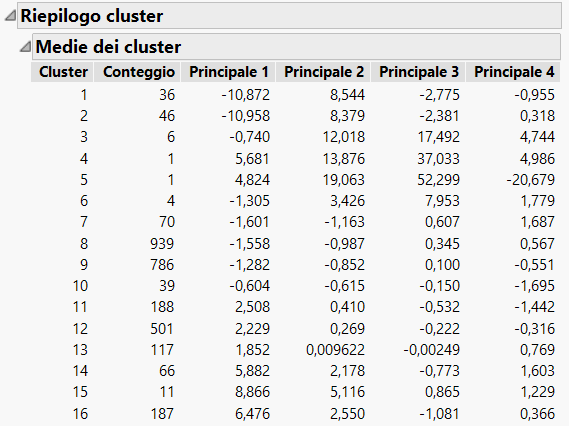
\includegraphics[width=0.30\textwidth]{Homework/Workload_Characterization/PCA_&_Clustering/4_Comp/Clustering/16_Cluster/Screen_Dati/Riepilogo.png}}
 	\caption{\textit{Numero di cluster e dimensione per diversi valori}}
 \end{figure}
La devianza persa durante la clusterizzazione varia in relazione al numero di cluster scelti. Si possono racchiudere le informazioni in un'unica tabella:
\begin{center}
	\begin{tabular}{|c|c|c|c|c|c|}
		\hline
		\textbf{6 Cluster} & \textbf{8 Cluster} & \textbf{10 Cluster} &\textbf{12 Cluster}& \textbf{14 Cluster} & \textbf{16 Cluster} \\
		\hline
		26\%& 17\% & 16\% & 15\% & 14.5\% & 14\% \\
		\hline
	\end{tabular}
\end{center}
\vspace{0.5cm}
 \subsection{5 Componenti Principali}
 Utilizzando le prime quattro PC si ha:
 \begin{figure}[H]
 	\centering   
 	\subfigure{	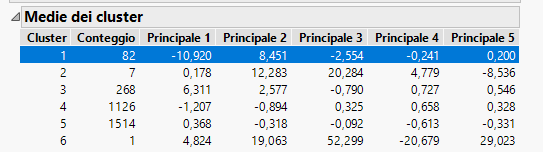
\includegraphics[width=0.30\textwidth]{Homework/Workload_Characterization/PCA_&_Clustering/5_Comp/Clustering/6_Cluster/Screen_Dati/Riepilogo.png}}
 	\subfigure{	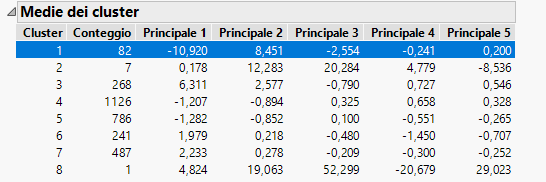
\includegraphics[width=0.30\textwidth]{Homework/Workload_Characterization/PCA_&_Clustering/5_Comp/Clustering/8_Cluster/Screen_Dati/Riepilogo.png}}
 	\subfigure{	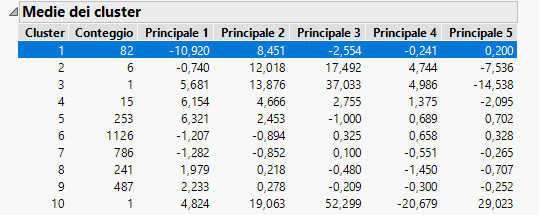
\includegraphics[width=0.30\textwidth]{Homework/Workload_Characterization/PCA_&_Clustering/5_Comp/Clustering/10_Cluster/Screen_Dati/Riepilogo.png}}
 	\subfigure{	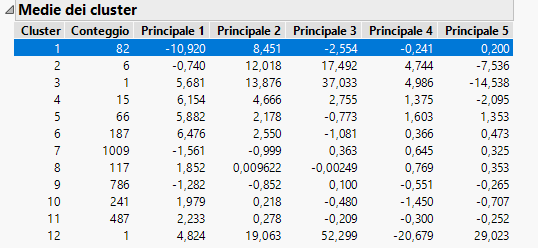
\includegraphics[width=0.30\textwidth]{Homework/Workload_Characterization/PCA_&_Clustering/5_Comp/Clustering/12_Cluster/Screen_Dati/Riepilogo.png}}
 	\subfigure{	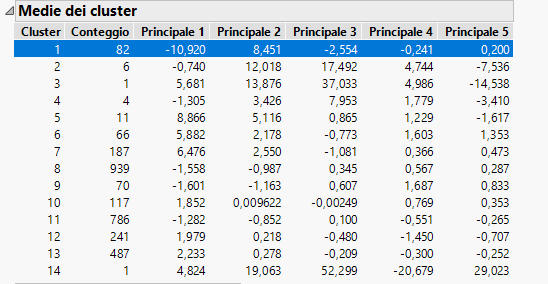
\includegraphics[width=0.30\textwidth]{Homework/Workload_Characterization/PCA_&_Clustering/5_Comp/Clustering/14_Cluster/Screen_Dati/Riepilogo.png}}
 	\subfigure{	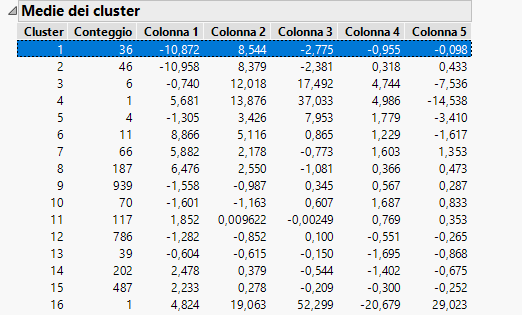
\includegraphics[width=0.30\textwidth]{Homework/Workload_Characterization/PCA_&_Clustering/5_Comp/Clustering/16_Cluster/Screen_Dati/Riepilogo.png}}
 	\caption{\textit{Numero di cluster e dimensione per diversi valori}}
 \end{figure}
La devianza persa durante la clusterizzazione varia in relazione al numero di cluster scelti. Si possono racchiudere le informazioni in un'unica tabella:
\begin{center}
	\begin{tabular}{|c|c|c|c|c|c|}
		\hline
		\textbf{6 Cluster} & \textbf{8 Cluster} & \textbf{10 Cluster} &\textbf{12 Cluster}& \textbf{14 Cluster} & \textbf{16 Cluster} \\
		\hline
		25.5\%& 16\% & 15\% & 12\% & 11\% & 10\% \\
		\hline
	\end{tabular}
\end{center}
\vspace{0.5cm}
 \subsection{6 Componenti Principali}
 Utilizzando le prime quattro PC si ha:
 \begin{figure}[H]
 	\centering   
 	\subfigure{	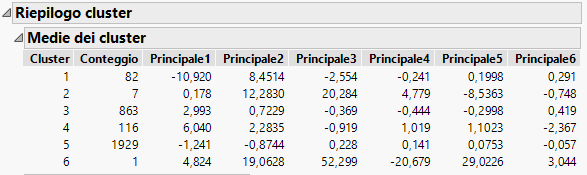
\includegraphics[width=0.30\textwidth]{Homework/Workload_Characterization/PCA_&_Clustering/6_Comp/Clustering/6_Cluster/Screen_Dati/Riepilogo.png}}
 	\subfigure{	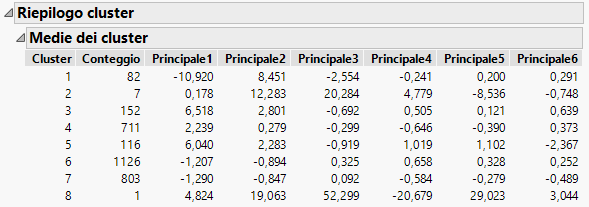
\includegraphics[width=0.30\textwidth]{Homework/Workload_Characterization/PCA_&_Clustering/6_Comp/Clustering/8_Cluster/Screen_Dati/Riepilogo.png}}
 	\subfigure{	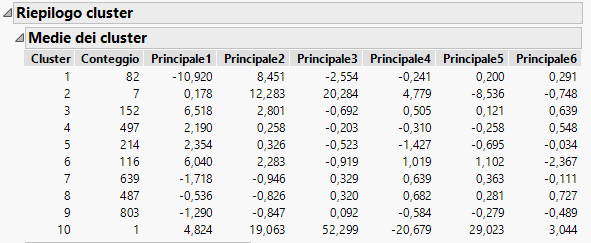
\includegraphics[width=0.30\textwidth]{Homework/Workload_Characterization/PCA_&_Clustering/6_Comp/Clustering/10_Cluster/Screen_Dati/Riepilogo.png}}
 	\subfigure{	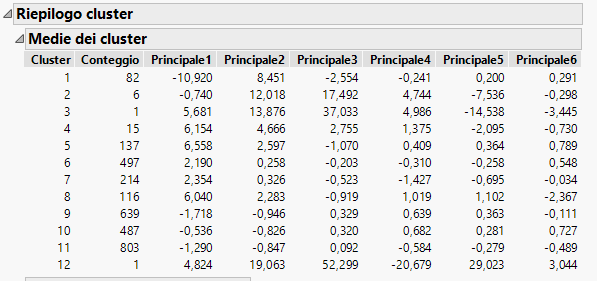
\includegraphics[width=0.30\textwidth]{Homework/Workload_Characterization/PCA_&_Clustering/6_Comp/Clustering/12_Cluster/Screen_Dati/Riepilogo.png}}
 	\subfigure{	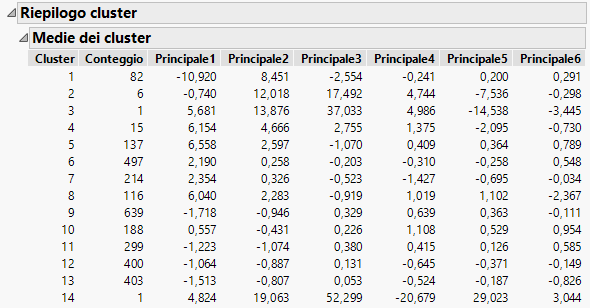
\includegraphics[width=0.30\textwidth]{Homework/Workload_Characterization/PCA_&_Clustering/6_Comp/Clustering/14_Cluster/Screen_Dati/Riepilogo.png}}
 	\subfigure{	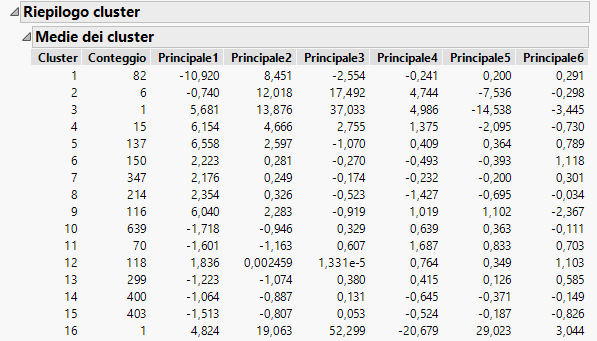
\includegraphics[width=0.30\textwidth]{Homework/Workload_Characterization/PCA_&_Clustering/6_Comp/Clustering/16_Cluster/Screen_Dati/Riepilogo.png}}
 	\caption{\textit{Numero di cluster e dimensione per diversi valori}}
 \end{figure}
 
 
 \begin{center}
 	\begin{tabular}{|c|c|c|c|c|c|}
 		\hline
 		\textbf{6 Cluster} & \textbf{8 Cluster} & \textbf{10 Cluster} &\textbf{12 Cluster}& \textbf{14 Cluster} & \textbf{16 Cluster} \\
 		\hline
 		22\% & 15\%& 13\% & 12\% & 11\% & 9\% \\
 		\hline
 	\end{tabular}
 \end{center}

\vspace{0.5cm}

\subsection{Interpretazione}
All'inizio dell'analisi sono state effettuate delle ipotesi che hanno trovato riscontro nella procedura di clustering:
\begin{enumerate}
	\item La fase iniziale del sistema (descritto dalle prime righe) trova riscontro con il cluster numero uno qualunque siano le componenti principali e qualunque sia il numero di cluster scelto. Questo quindi prova l'ipotesi definita inizialmente
	\item L'ultimo cluster contiene sempre un elemento singolo. Questo accade a causa del fatto che è stato identificato un picco nella fase iniziale delle misure. Esso inoltre è stato definito grazie all'outlier nel parametro Slab che non è stato eliminato, di conseguenza il picco viene racchiuso in un unico cluster in tutte le situazioni.
\end{enumerate}
\vspace{0.5cm}
In conclusione si può costruire una tabella che racchiude le informazioni riguardanti le PCA e la clusterizzazione in termini di percentuale di devianza persa.
 \begin{center}
	\begin{tabular}{|c|c|c|c|c|c|c|}
		\hline
		& \textbf{6 Cluster} & \textbf{8 Cluster} & \textbf{10 Cluster} &\textbf{12 Cluster}& \textbf{14 Cluster} & \textbf{16 Cluster} \\
		\hline
		\textbf{4 PC} & 26\%& 17\% & 16\% & 15\% & 14.5\% & 14\% \\

	\textbf{5 PC} & 25.5\%& 16\% & 15\% & 12\% & 11\% & 10\% \\

		\textbf{6 PC} & 22\% & 15\%& 13\% & 12\% & 11\% & 9\% \\
		\hline
	\end{tabular}
\end{center}

\newpage
\section{Workload Sintetico}
Come anticipato nel paragrafo precedente, sono state scelte 5 PC e per non perdere troppa varianza ma al tempo stesso non sfociare in un numero di cluster molto elevato, si è scelto di considerare 10 cluster. In tal caso la perdita di devianza con PCA e Cluster è di circa del 15\%.
\\In conclusione dopo aver calcolato i centroidi con uno script MATLAB il workload sintetico risulta essere:
\begin{figure}[H]
	\centering
	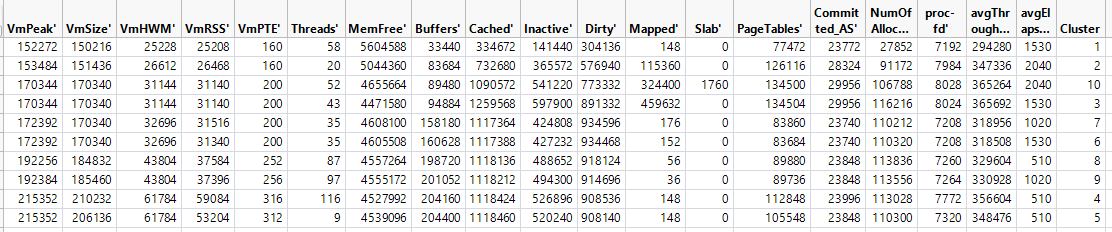
\includegraphics[width=\textwidth]{img/hw1/workload_sintetico.png}
	\caption{\textit{Workload sintetico}}
\end{figure}
	\chapter{Web Server - Capacity Test}
L'obiettivo del Capacity Test è quello di valutare le performance di un qualsiasi sistema quando è sottoposto a carichi di lavoro di diversa intensità, in modo da caratterizzare le sue prestazioni al limite (sotto condizioni di lavoro severe).
\\
Per realizzare queste valutazioni sono necessari gli \textbf{high-level parameters}, ovvero tutti quei parametri reperibili ed osservabili lato client. Essi possono riferirsi alla richiesta (quando è stata fatta, chi l'ha fatta ecc..) o alla risposta (tempi di risposta, errori).
\\
Essendo il sistema in questione un server, si è scelto di descrivere le sue performance attraverso:
\begin{enumerate}
	\item \textbf{Response Time}, intervallo di tempo che intercorre tra l'istante in cui il client inoltra la richiesta e quello in cui riceve la risposta.
	\item \textbf{Throughput}, richieste servite correttamente per unità di tempo.
\end{enumerate}
L'andamento atteso da parte di queste due metriche è il seguente:
\begin{figure}[H]
	\centering
	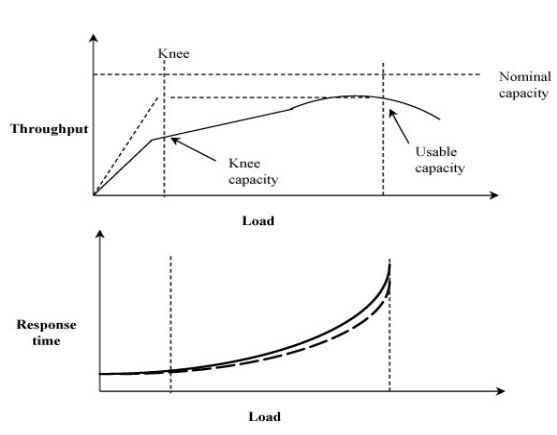
\includegraphics[width=0.8\textwidth]{img/hw2/Thr_resp.png}
	\caption{\textit{Grafici Throughput e Response time}}
\end{figure}
Di nostro interesse sono i valori di:
\begin{itemize}
	\item \textit{Knee Capacity}, punto prima del quale il throughput cresce linearmente all'aumentare del carico, ma il tempo di risposta non varia significativamente ed oltre il quale il guadagno in throughput è basso mentre il tempo di risposta aumenta con il carico.
	\item \textit{Usable Capacity}, massimo throughput raggiungibile portando il sistema al limite, senza eccedere un dato tempo di risposta.
\end{itemize}
Per ottenere agevolmente la Knee Capacity, viene introdotto un terzo parametro, la \textit{Potenza}. 
\\
\begin{equation}
	Power = \frac{Throughput}{Response Time}
\end{equation}
Tale punto coincide con il punto di massimo della potenza e rappresenta l'ottimo in corrispondenza del quale conviene operare per ottenere le prestazioni migliori.
\begin{figure}[H]
	\centering
	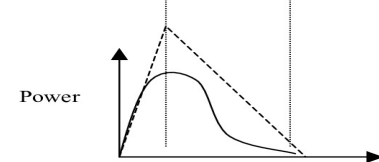
\includegraphics[width=0.5\textwidth]{img/hw2/Power.png}
	\caption{\textit{Grafico Potenza}}
\end{figure}


\section{Experimental Setup}
Il sistema oggetto di studio è un \textit{Web Server Apache} installato sulla macchina virtuale guest, che funge da server.
\\
Tramite la modalità \textit{Host-only Network Adapter}, configurabile nelle impostazioni della macchina virtuale, è stato possibile far comunicare la macchina guest con quella host, che lo ospita. Su quest'ultima è stata installata l'applicazione Java \textit{JMeter}, che ha permesso l'analisi delle prestazioni complessive del Server, sottoponendolo a diversi tipi di carico.
\\
\\
In questa analisi è stato scelto di valutare le prestazioni in media del server, considerando solo richieste (HTTP di tipo GET) casuali. Esse sono differenziate dalla dimensione della risorsa che chiedono al server. 

\subsection{Server Setup}
Il server è stato installato su una macchina virtuale \textit{Ubuntu 2021} in esecuzione su una macchina host di uso comune. Essa è stata dotata di circa 4GB di RAM e di 2 processori (intel I5-5200u con frequenza massima di 2.70 GHz).
\\Per creare un scenario reale, sul Server sono state caricate 5 pagine in formato testuale, di diversa dimensione:
\begin{itemize}
	\item \textbf{Small}: 50 KB
	\item \textbf{Small-Medium}: 100 KB
	\item \textbf{Medium}: 300 KB
	\item \textbf{Medium-Large}: 500 KB
	\item \textbf{Large}: 1 MB
\end{itemize}
Questi sono i file oggetto delle richieste realizzate da ipotetici client.

\subsection{Clients Setup - JMeter}
Innanzitutto è stato settato, nel \textit{ThreadGroup}, il numero di thread che JMeter usa per realizzare i test. Questa quantità rappresenta il numero di utenti "virtuali" che visitano il nostro server. Nel nostro esperimento sono stati previsti \textbf{50 threads}, un valore in linea con i suoi scopi (dato che si tratta di un banale webserver virtualizzato su una macchina host di uso comune). In più, prevedendo dei test di durata pari a \textit{5 min}, sono stati impostati:
\begin{itemize}
	\item il \textbf{Ramp-up period} - numero di secondi entro il quale deve essere attivato l'ultimo thread - a \textit{300 s}. Ciò ci ha permesso di dilazionare l'attivazione degli utenti nei 5 minuti.
	\item il \textbf{Thread lifetime} - durata massima di ogni thread - a \textit{300 s}.
	\item il \textbf{Loop count} - numero di volte in cui un singolo thread effettua una richiesta. Esso corrisponde al numero di richieste nell'intervallo di tempo di simulazione (in questo caso 300s) diviso il numero di threads.
\end{itemize}
Al ThreadGroup sono stati aggiunti 5 \textit{HTTP Request Sampler}, uno per tipologia di richiesta da realizzare e nei quali sono stati specificati i path delle rispettive risorse sul server. Ad essi è stato integrato un \textit{Random Controller}, grazie al quale, quando un thread viene attivato, effettua solo una tra le cinque tipologie di richieste, selezionata in maniera randomica. Ancora una volta, aggiungendo variabilità alle nostre richieste, è stato possibile simulare una situazione realistica e, soprattutto, non predicibile.
\\
Attraverso il \textit{Constant Throughput Timer} è stato possibile impostare il carico da sottoporre al sistema, in termini di numero di richieste al minuto. Infine, il listener \textit{Simple Data Writer}, ci ha permesso di collezionare in un file, quei parametri di alto livello che sono d'interesse ai fini dell'esperimento.
\\L'idea è quella di simulare quindi 50 utenti, di cui ognuno effettua un numero di richieste in relazione al carico, per 5 min. \\Ciò equivale a:
\begin{figure}[H]
	\centering
	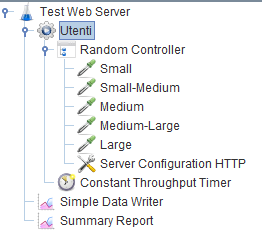
\includegraphics[width=0.4\textwidth]{img/hw2/jmeter.png}
	\caption{\textit{Configurazione delle richieste e del carico in JMeter}}
\end{figure}
I risultati, grazie al Simple Data Wirter, vengono salvati in formato .csv, i cui paramentri vengono raggruppati in forma tabellare.
\begin{center}
\begin{tabular}{|l|l|l|l|}
	\hline
	TimeStamp & Elapsed & Latency & ... \\
	\hline
	\vdots &  \vdots & \vdots & \vdots \\
	\hline
\end{tabular}
\end{center}
\section{Esecuzione Capacity Test}
Inizialmente sono stati effettuati dei test il cui scopo era quello di far operare il Web Server "al limite". Ci si è resi conto che il massimo valore di carico entro il quale il sistema risponde adeguatamente (in quelle condizioni), è di circa \textit{6000 richieste al minuto}. 
\\
A partire da questo limite e ragionando sull'andamento di throughput e response time, si sono scelti i seguenti valori di carico da sottoporre al sistema:
\begin{equation*}
	workloads = {100, 500, 800, 1000, 2000, 3000, 4000, 5000, 6000, 7000, 8000, 9000}
\end{equation*}
Gli ultimi tre carichi (7000, 8000 e 9000 richieste al minuto) hanno permesso di evidenziare nei grafici il degradamento delle prestazioni del sistema.
\\
Per ogni valore di carico è stato calcolato il \textbf{Throughput}:

\begin{equation}
	Throughput = \frac{NumeroRichieste}{Timestamp(N) - Timestamp(1)} \quad  \left[ \frac{N}{s} \right] 
\end{equation}
Il \textit{timestamp} fa parte degli high-level parameters collezionati dal Simple Data Writer, e corrisponde all'istante di tempo (in millisecondi poi convertito in secondi) in cui il client ha inoltrato una data richiesta.
\\
Come \textbf{Response Time} è stato scelto il parametro \textit{Elapsed}, coincidente con il tempo che intercorre tra la sottomissione della richiesta da parte del client e la risposta del server. Dato che contiene anche il tempo di elaborazione della richiesta da parte del server, esso cresce all'aumentare della dimensione dei file richiesti, oltre che all'aumentare del carico.
\\
\\
Ogni misurazione (per ogni carico) è stata ripetuta \textbf{3 volte} in modo da tenere traccia dell'errore, e notando che i dati ottenuti non differivano di molto tra loro, come indice di posizione è stata scelta la loro media.
\\
\subsection{Risultati}
I file .csv sono stati caricati in uno script Matlab tramite cui sono stati automatizzati i procedimenti descritti sopra, i parametri sono stati plottati in funzione del carico considerato.
differenziale).
\begin{minted}[framesep = 1mm,
	fontsize = \footnotesize,
	breaklines,
	]{MATLAB}
%% Data
workloads = [100 500 800 1000 2000 3000 4000 5000 6000 7000 8000 9000];
througputs = zeros(1, length(workloads));
resp_times = zeros(1, length(workloads));
k = 1; %Indice di riferimento per i due vettori

%% Elaborazione
for i = workloads
	mean_resp_t = zeros(1,3);
	thr = zeros(1,3);
	for j = 1:3
		path = strcat(num2str(i, '%d'),'\dati',num2str(j,'%d'),'.csv');
		
		%Data from Jmeter output file (csv format)
		simple_data = readmatrix(path);
		
		%Calculating the number of requests
		[N, M] = size(simple_data);
		num_req = N; %Number of requests
		
		%Throughput = number_of_requests_completed / time_window_of_the_experiment
		t_wind_mills = simple_data(num_req,1) - simple_data(1,1); %Time window (milliseconds)
		t_wind_sec = t_wind_mills/1000; %Time window (seconds)
		thr(j) = num_req/t_wind_sec; %Throughput
		
		%Average response time
		elap_times = simple_data(:,2);
		mean_resp_t(j) = mean(elap_times);
	end

	check deviazione_std    
	COV_thr(k) = std(thr)/mean(thr);
	COV_resp(k) = std(mean_resp_t)/mean(mean_resp_t);
	     
	if COV_thr(k) > 0.5     
		througputs(k) = median(thr);
	end

	if COV_resp(k) > 0.5
		resp_times(k) = median(mean_resp_t);
	end

end

power = througputs./(resp_times/1000);
power_max = max(power);
KNEE_CAPACITY = througputs(find(power == power_max));
\end{minted}
Effettuando un grafico dei risultati:
\begin{figure}[H]
	\centering
	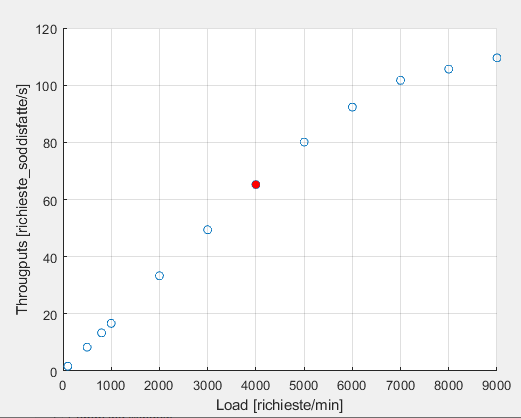
\includegraphics[width=0.8\textwidth]{img/hw2/Throughput.png}
	\caption{\textit{Grafico Throughput}}
\end{figure}

\begin{figure}[H]
	\centering
	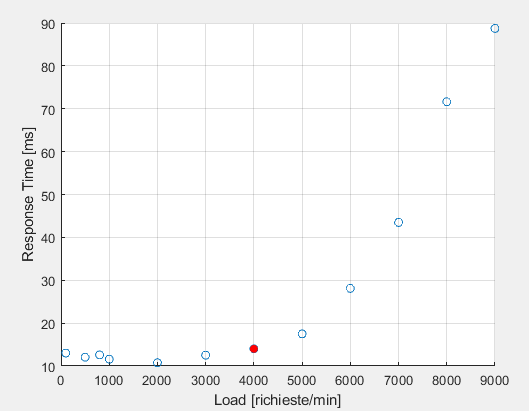
\includegraphics[width=0.8\textwidth]{img/hw2/ResponseTime.png}
	\caption{\textit{Grafico Response Time}}
\end{figure}

\begin{figure}[H]
	\centering
	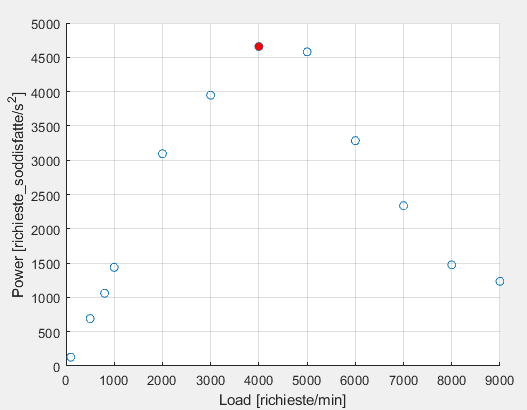
\includegraphics[width=0.8\textwidth]{img/hw2/Potenza.png}
	\caption{\textit{Grafico Potenza}}
\end{figure}
\newpage

Come si evince dal grafico della Potenza, il suo punto di massimo è associato ad un carico di 4000 richieste/min. 
\\
La \textit{Knee Capacity} (in rosso nel grafico dei Throughputs) è il valore throughput associato a questo carico. Ciò significa che se il nostro server opera in condizioni ottimali riesce a soddisfare circa 65,2112 richieste al secondo, ovvero 3836 richieste al minuto mediamente.
\\

Per quanto riguarda il calcolo della \textit{Usable Capacity}, possiamo relazionarla al tempo di risposta del server quando è sottoposto ad un carico di 6000 richieste/min (il carico limite). Questo response time è pari a 28,11 ms e coincide con quel tempo oltre il quale il sistema inizia a non rispondere più adeguatamente. Pertanto, la Usable Capacity può essere espressa come il valore di throughput associato al carico limite, ovvero 92,3314 richieste al secondo (5431 richieste al minuto circa).
\\
Ovviamente il valore di carico a cui conviene far lavorare il nostro Web Server non è quello massimo che riesce a soddisfare (Usable Capacity). Difatti non sarebbe efficiente per due motivi:
\begin{enumerate}
	\item I tempi di risposta associato a tale carico sono elevati.
	\item Essendo il carico limite, bastano poche richieste in più per ricadere nella zona in cui i tempi di risposta diventano estremamente elevati, rendendo inutilizzabile il server stesso. 
\end{enumerate}

	\backmatter							%Fine numerazione capitoli (Per le conclusioni, Appendici ecc)
	

	
\end{document}